\section{Volatility}
\subsection{Business Series}
% \begin{lstlisting}[language=R]
% acf(resid(y1.sarima)^2, main="Squared Residuals")
% \end{lstlisting}
\begin{figure}[H]
    \centering
    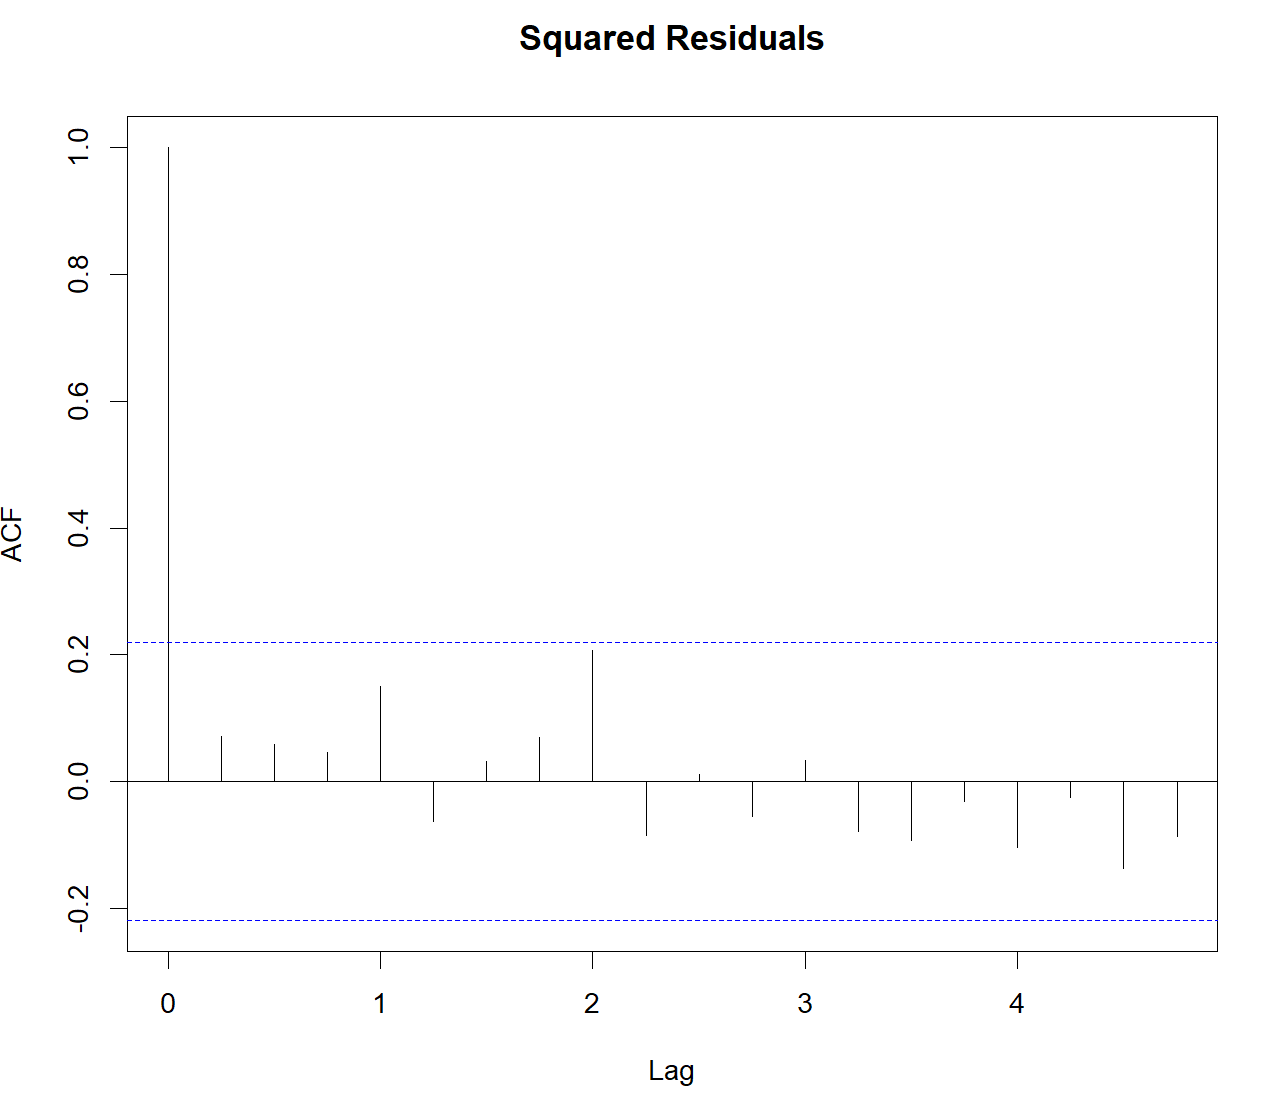
\includegraphics[width=0.6\linewidth]{fig/y1sq.png}
\end{figure}
The correlogram of the squared residuals shows no significant values, so there is no evidence of conditional heteroskedastic behaviour or volatility in the residual series, and an ARCH or GARCH model is not required.

\subsection{Holiday Series}
\begin{figure}[H]
    \centering
    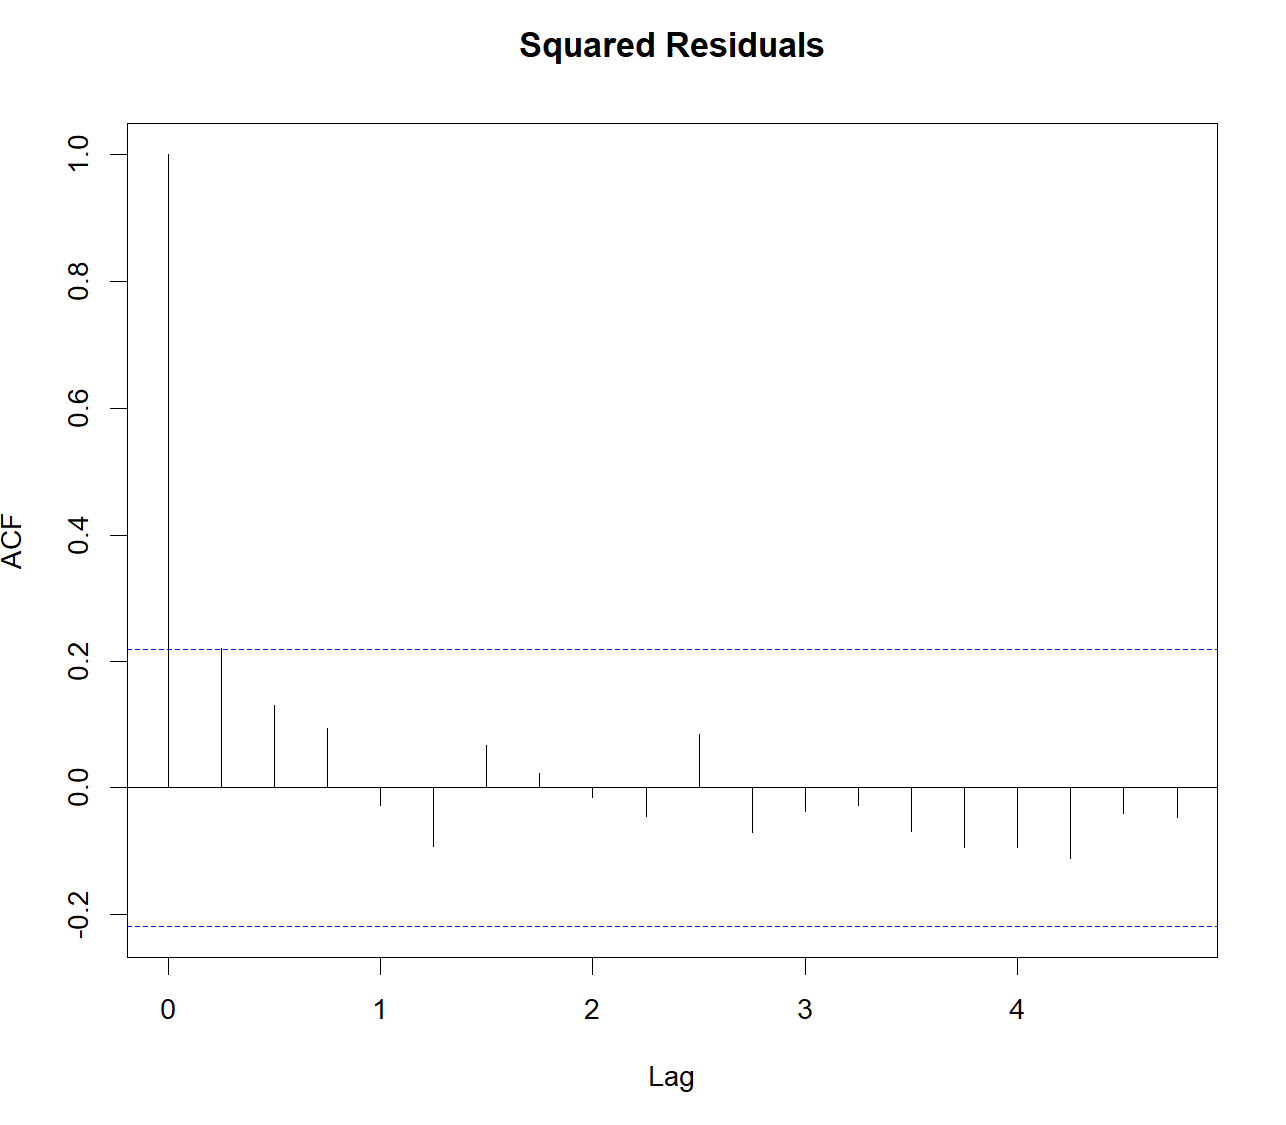
\includegraphics[width=0.6\linewidth]{fig/y2sq.png}
\end{figure}

The correlogram of the squared residuals does not show any significant spikes, which suggests that the residual variance remains relatively stable over time. There is no clear evidence of conditional heteroskedasticity or volatility clustering in the Holiday series. Therefore, a GARCH-type model is not necessary.

\subsection{Conclusion of the Two Series}

\noindent For the both Business and Holiday series shows that the squared residual correlograms do not show significant values. This suggests that both models have relatively stable residual variance and no strong volatility clustering. Hence, an ARCH or GARCH-type model is unnecessary for both series.

